% This is LLNCS.DEM the demonstration file of
% the LaTeX macro package from Springer-Verlag
% for Lecture Notes in Computer Science,
% version 2.4 for LaTeX2e as of 16. April 2010
%
\documentclass{article}
%
\usepackage{makeidx}  % allows for indexgeneration
\usepackage{amsmath}
\usepackage{graphicx}
\usepackage{color}
\usepackage{transparent}
\usepackage{pbox}
\usepackage{pgfplots}
\usepackage{listings}


\usepackage{listings}
\usepackage{graphicx} 
\usepackage{subcaption}  



\usetikzlibrary{calc} 
\pgfplotsset{compat=1.8}
%\usepackage{array}
%

\begin{document}

%
\pagestyle{headings}  % switches on printing of running heads
%\addtocmark{Hamiltonian Mechanics} % additional mark in the TOC
%
%\tableofcontents
%

%

\title{Automatic length and angle calculation of DNA on AFM images}

\author{Insert authors' names here}

\maketitle  
\newpage
\tableofcontents
\newpage
%
\begin{abstract}
	This report summarizes ...
	
\end{abstract}

\section{Introduction}
This is how you cite \cite{ficarra2005automated}.
The sources are saved in sources.bib. If you find a paper/article/book on googlescholar, click "cite" and copy the bibtex cite style into the source file. It will looks something like this:
\begin{verbatim}
@article{ficarra2005automated,
  title={Automated DNA fragments recognition and sizing through AFM image processing},
  author={Ficarra, Elisa and Benini, Luca and Macii, Enrico and Zuccheri, Giampaolo},
  journal={Information Technology in Biomedicine, IEEE Transactions on},
  volume={9},
  number={4},
  pages={508--517},
  year={2005},
  publisher={IEEE}
}
\end{verbatim}
Alternatively just save them in a text document and we will merge all of them in the end. 




\section{Methods}
This is how you include tables:
\begin{table}[htb]
	\begin{center}
		\caption{My Table Caption.}
		\label{tab: example} % you need to include this to reference the table afterwards
		\begin{tabular}{|l|l|l|l|l|l|}
			\hline
			x & y & z & $\alpha$
			& $\beta$
			& $\gamma$\\\hline
			30  & 0.82 & 38.4 & 35.7 & 154 & 320 \\
			60  & 0.67 & 42.1 & 34.7 & 138 & 340 \\
			120 & 0.52 & 45.1 & 34.0 & 124 & 370 \\
			\hline
		\end{tabular}
	\end{center}
\end{table}\\
And this is how you reference a table: See Table \ref{tab: example}.\\



















\subsubsection{Adaptive Thresholding}
The TIFF images often vary in intensity, distribution and scaling of the height profile of the DNA samples. This presents a couple of problems for the thresholding algorithms, such as pollution of some image regions which distort the threshold. As discussed here (\ref{sec:Thresholding}) these issues lead to a false classification of the DNA strands up to completely falsifying the results on this image.
Two sorts of noise persist after the initial pipelining steps  
Opencv Denoising, LowPassFilter and Median Filter(see section \ref{sec:Filtering}).
\begin{figure}[!htb]
	\begin{subfigure}{0.5\textwidth}
		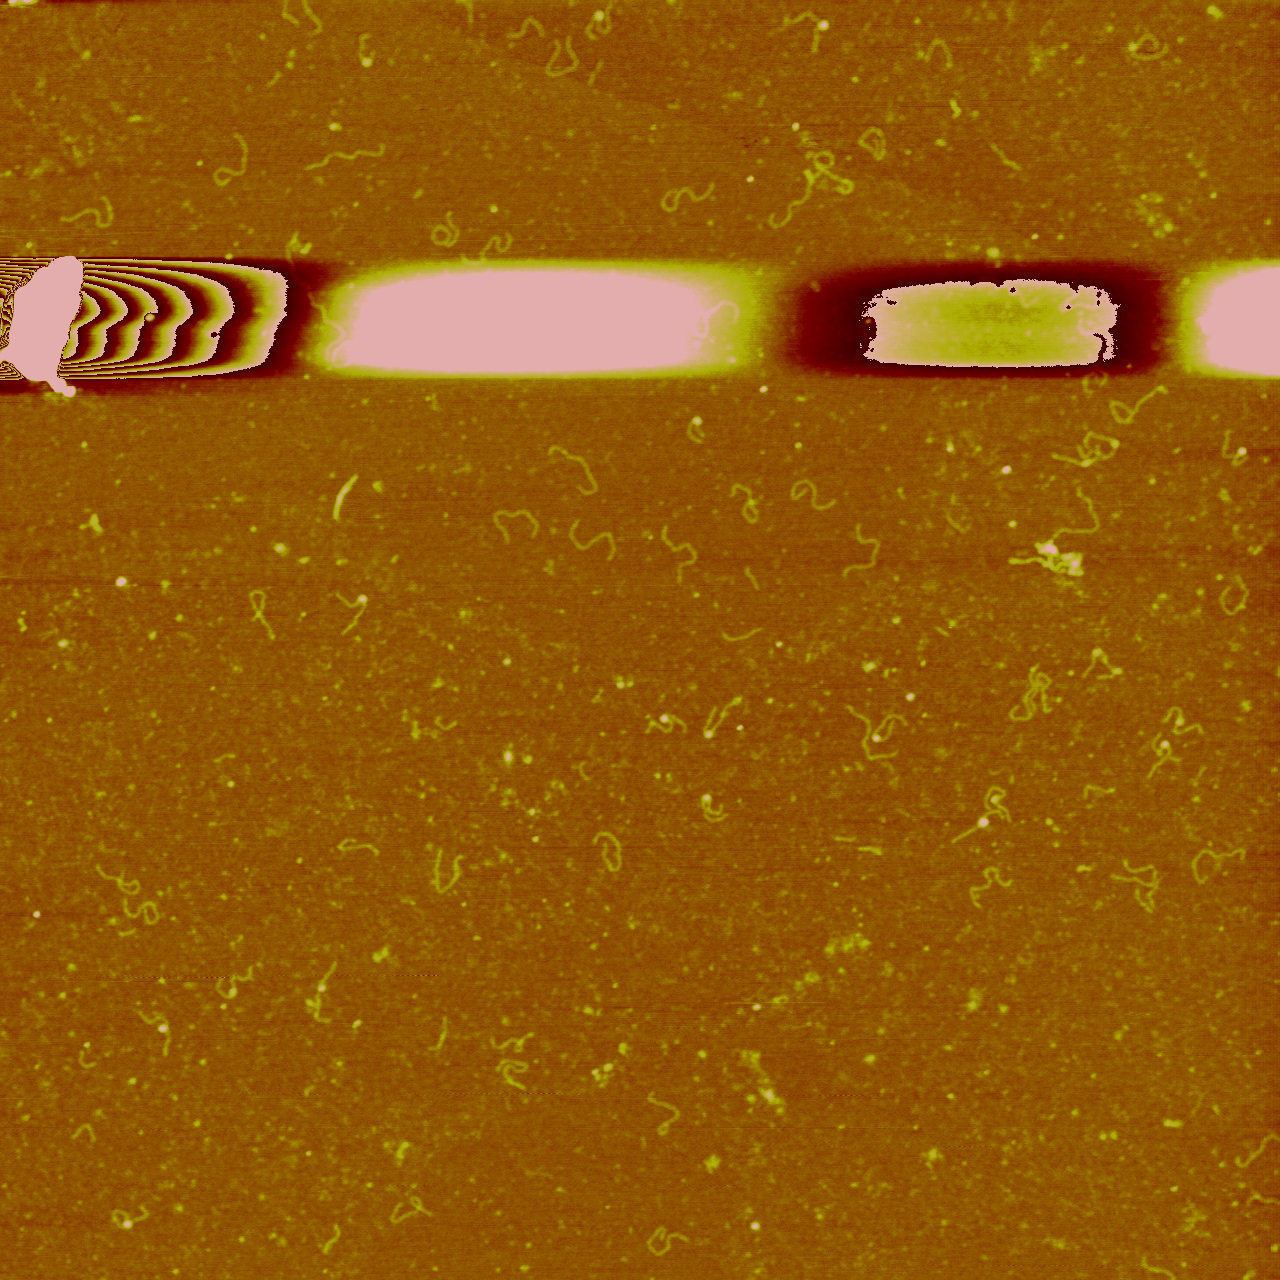
\includegraphics[width=\linewidth]{noise1.png}
		\caption{}
		\label{fig: Noise1}
	\end{subfigure}%
	\hspace{\fill}
	\begin{subfigure}{0.5\textwidth}
		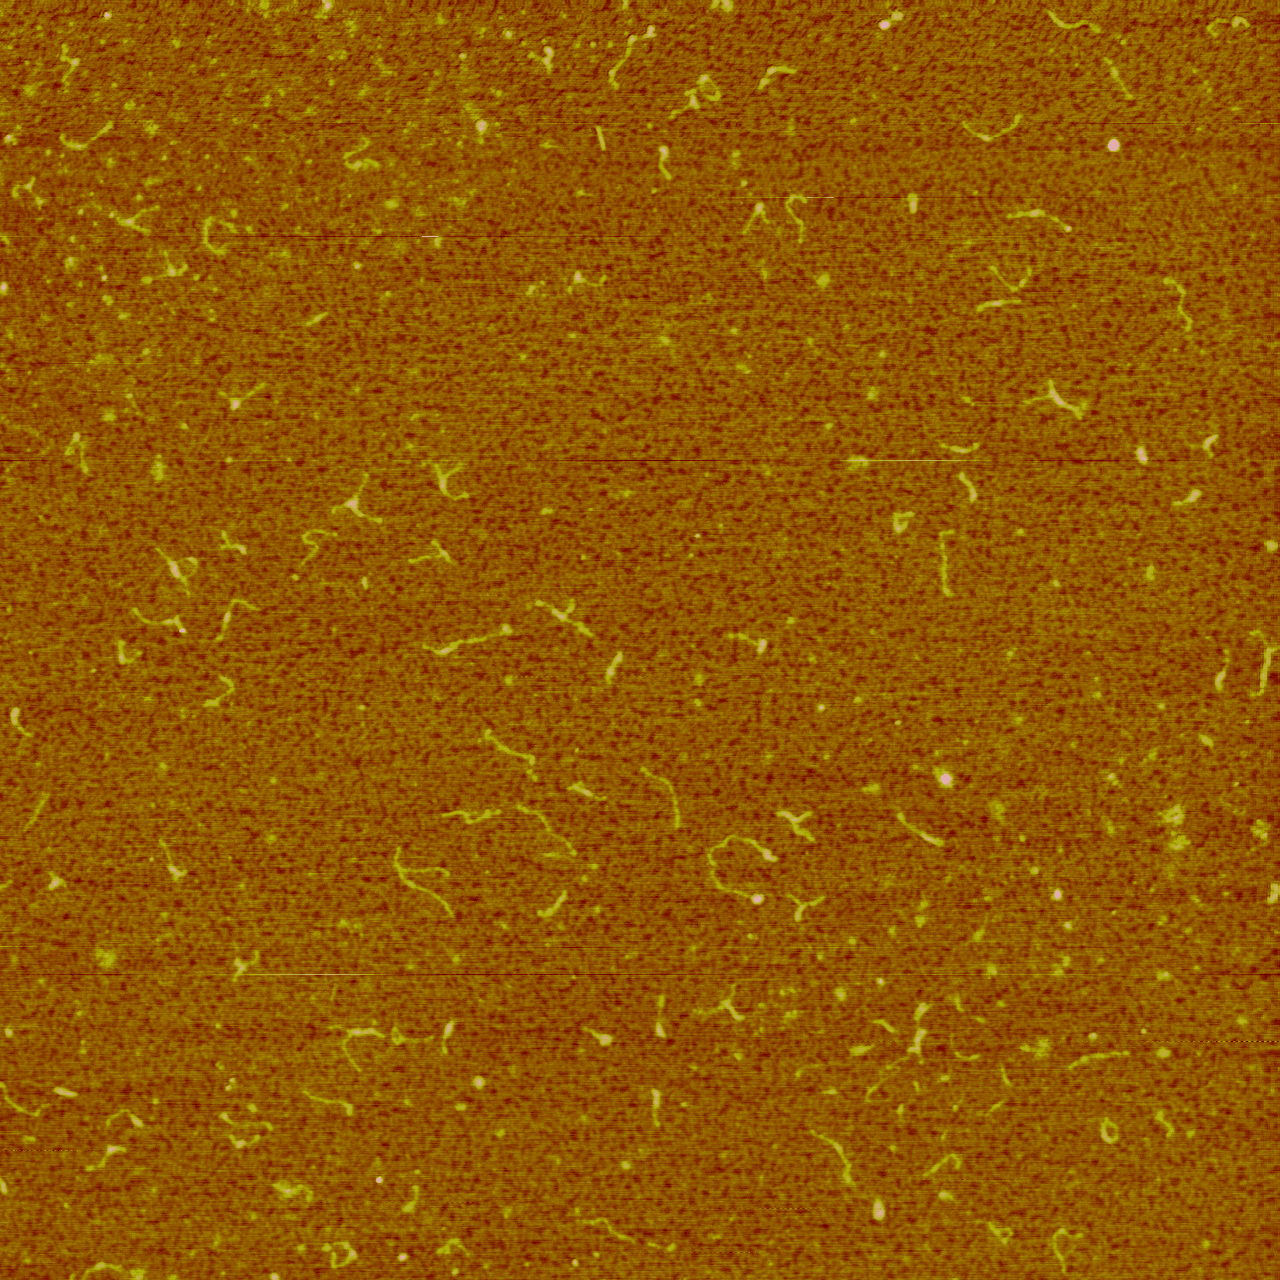
\includegraphics[width=\linewidth]{noise2.png}
		\caption{}
		\label{fig: Noise2}
	\end{subfigure}%
	\caption{(a)Noise Example 1 (b)Noise Example 2}\label{fig:Noise1Noise2}
\end{figure}
\\
The first type of noise as seen in Figure \ref{fig: Noise1} are large distorted regions in the upper value range at an approximate height of 190. If not handled these regions lift the threshold to a level where DNA-strands are missed entirely. 
The second sort of noise seen in Figure \ref{fig: Noise2} consists of small imperfections scattered over the whole image.
Unfortunately the height profile of these imperfections is very similar to the one of the DNA-strands and it is therefore very hard to automatically distinguish between them.
The overwhelming majority of disturbance on the images observed is part of the first type.
The aim of this part of the pipeline is to pre-process the data by three additional steps which treat the outliers in the upper value range and if possible improve detection and removal of scattered noise.

In order to tackle these issues the following three step method is proposed:
\begin{enumerate}
	\item Homogenize the background to provide a consistent and distinguishable layer on which the DNA-strands can be recognized easily.
	\item Identify and remove polluted image regions and outliers in the upper intensity values.
	\item Limit the threshold to an appropriate range.
\end{enumerate}
\subsubsection{Level Background}

Figure \ref{fig:HistThresh} shows a histogram of the height values of a representative original image from the dataset.
In the observed dataset DNA-strands can only be found in an intensity range from about 110 to 160, while nuclei can be found between 160 and 200.


\begin{figure}[!htb]
	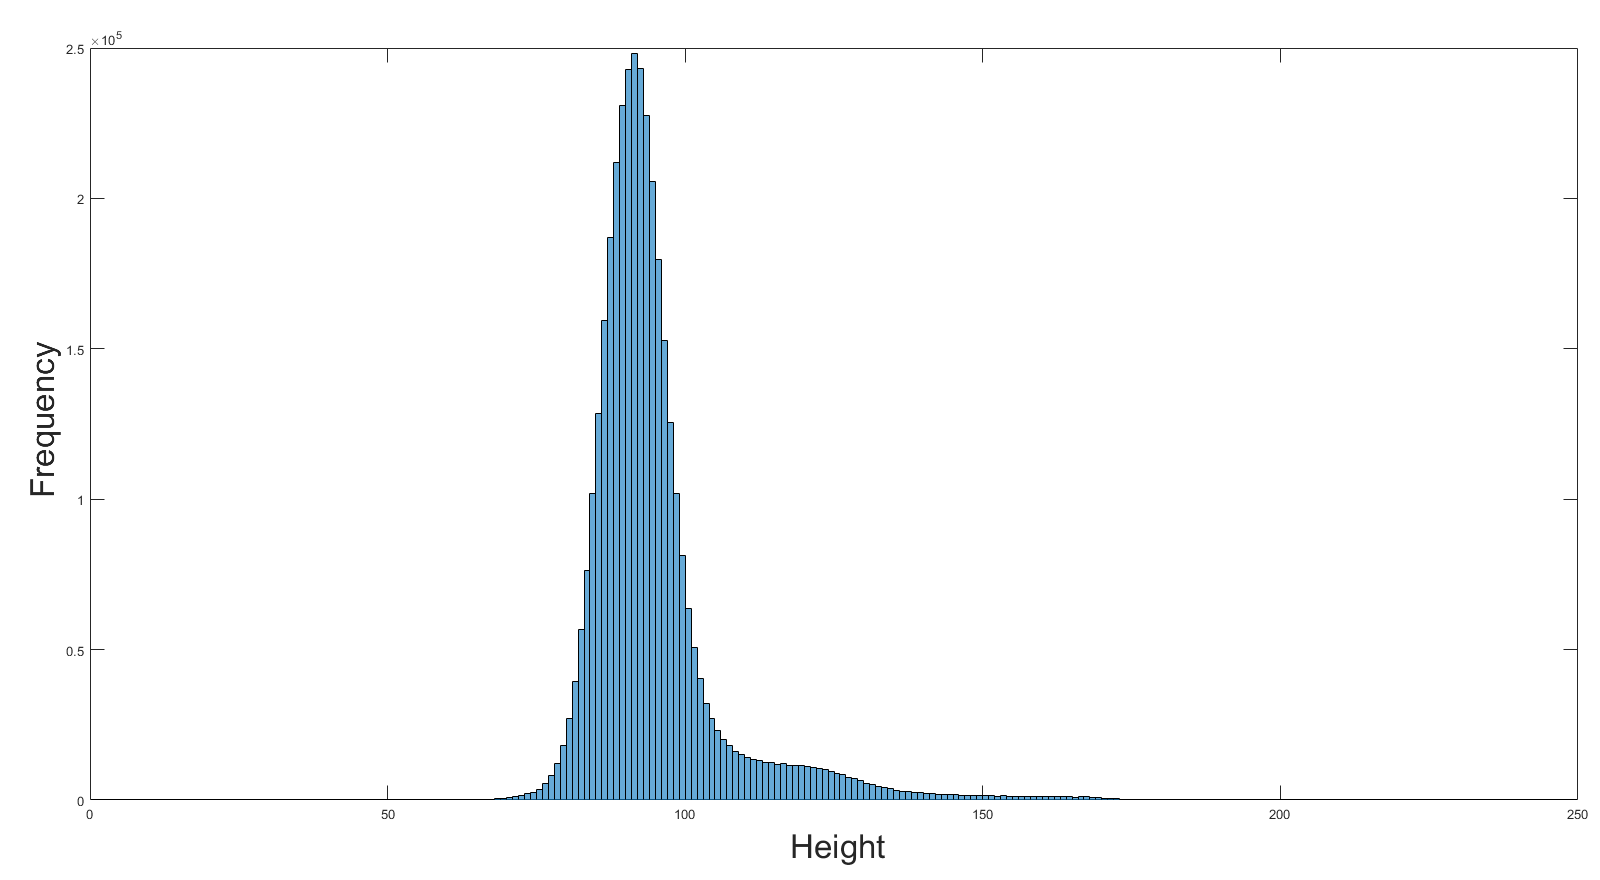
\includegraphics[width=1\linewidth]{histogramOriginal.png}
	\caption{Histogram of TIFF image}
	\label{fig:HistThresh}
\end{figure}
The accumulation point at a value of 95 is distinctive for background noise. 
Therefore, smaller values are set to this boundary.
This approach creates a more consistent background for all images and limits the variation due to noise.
It is important to mention that this method can only be used after the lowPassFilter(see section \ref{Adaptive Lowpass Filter}) which smooths the height distribution and thereby guarantees that only noise is removed. If applied to the raw unfiltered image this method will also remove outliers within the DNA-strands which results in perforated DNA objects.
The resulting image shown in Figure \ref{fig:background} yields a more consistent threshold and with that a higher resistance to image pollution.


\begin{figure}[!htbp]
	\begin{subfigure}{0.5\textwidth}
		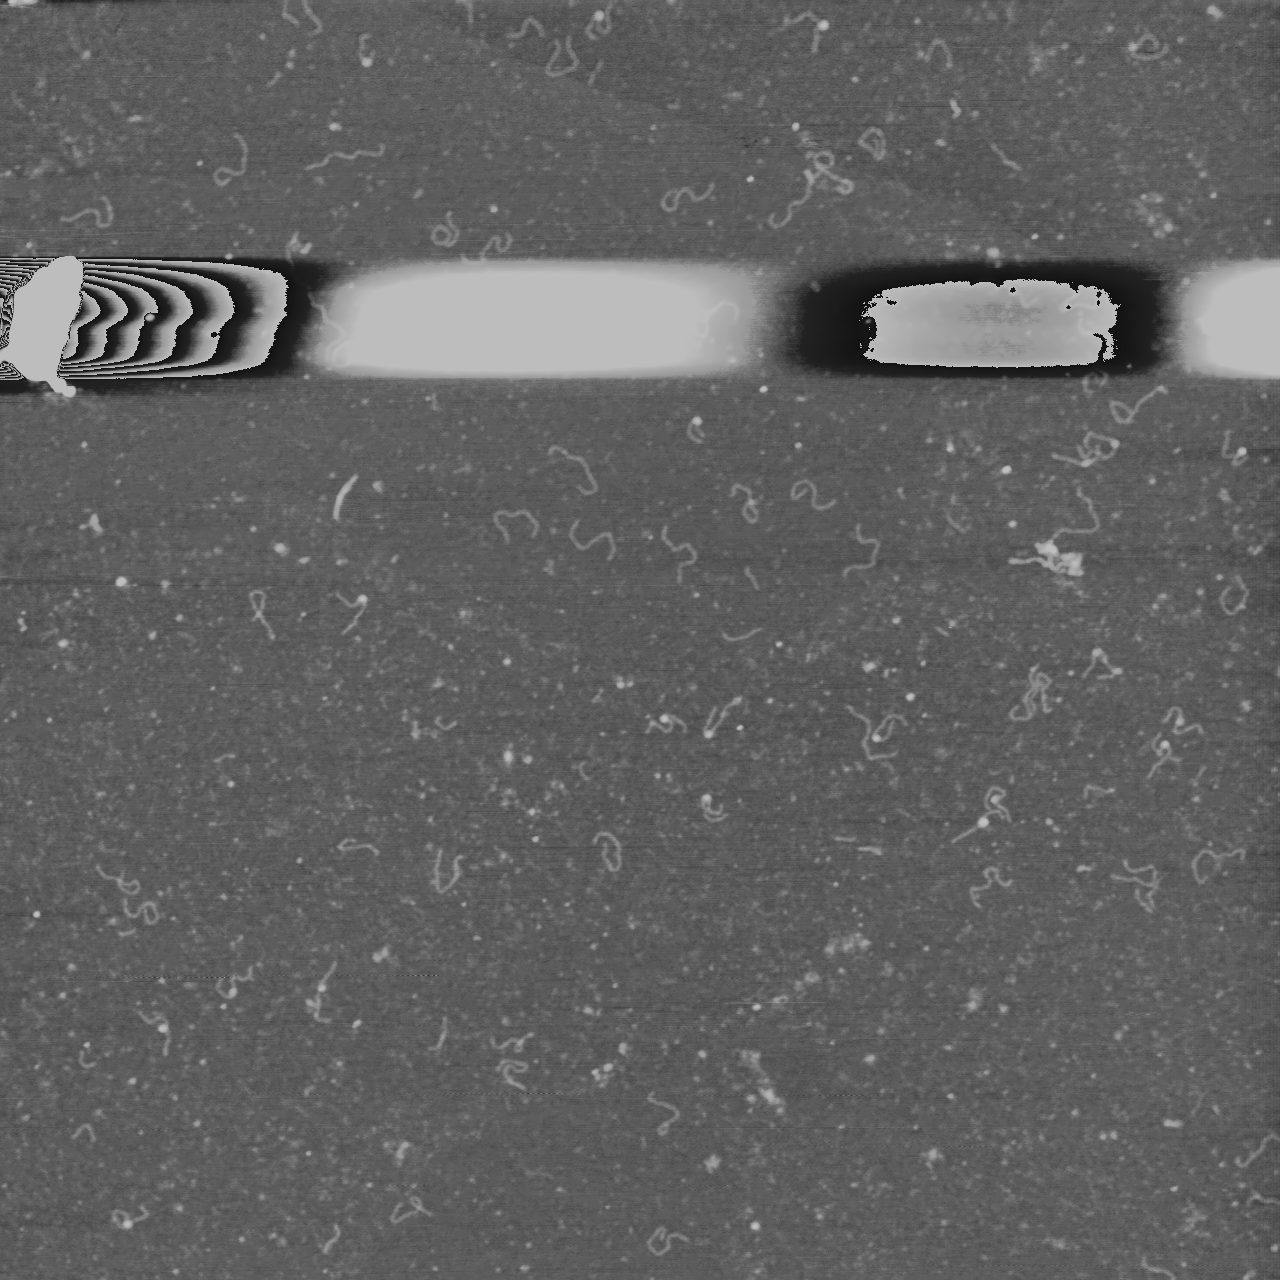
\includegraphics[width=\linewidth]{noise21.png}
		\caption{}
		\label{fig:rawImage}
	\end{subfigure}%
	\hspace{\fill}
	\begin{subfigure}{0.5\textwidth}
		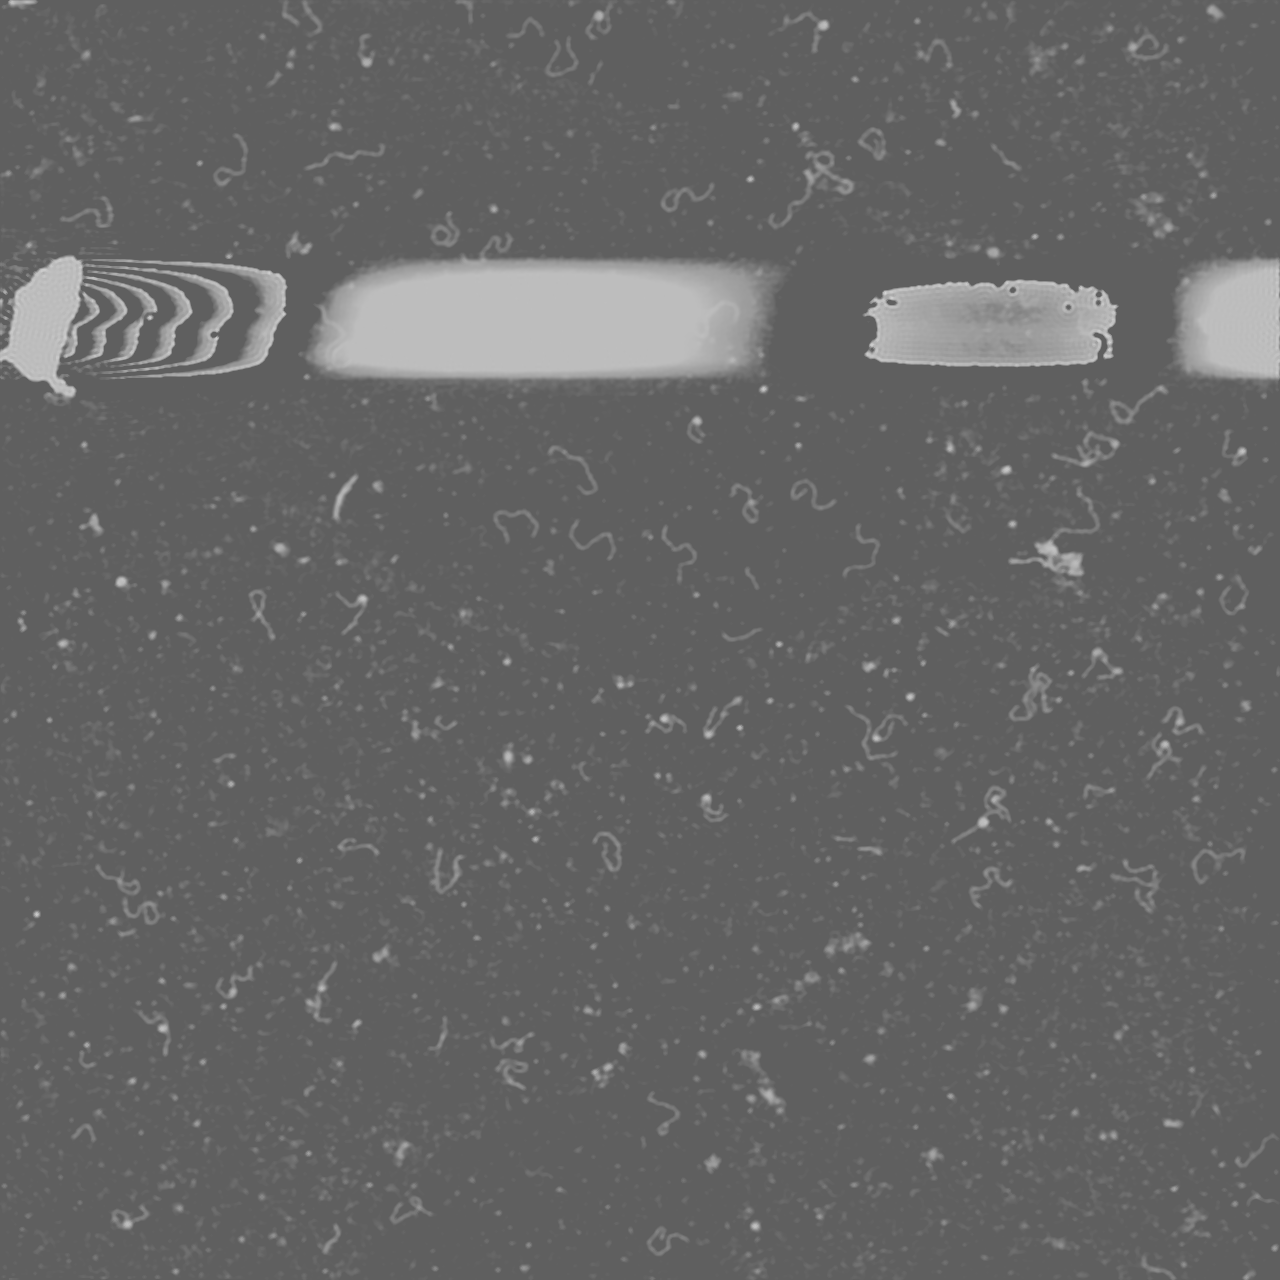
\includegraphics[width=\linewidth]{step21.png}
		\caption{}
		\label{fig:step1}
	\end{subfigure}%
	\caption{(a)Before leveling (b)After leveling }\label{fig:background}
\end{figure}
\subsubsection{Identify and remove outliers}
At first a global threshold algorithm like the Otsu method (see section \ref{sec:Thresholding}) is used to create a binary image.
All objects that could be a DNA object are removed based on size. Now only noise and other non-DNA objects are left.

\begin{figure}[!htb]
	\begin{subfigure}{0.5\textwidth}
		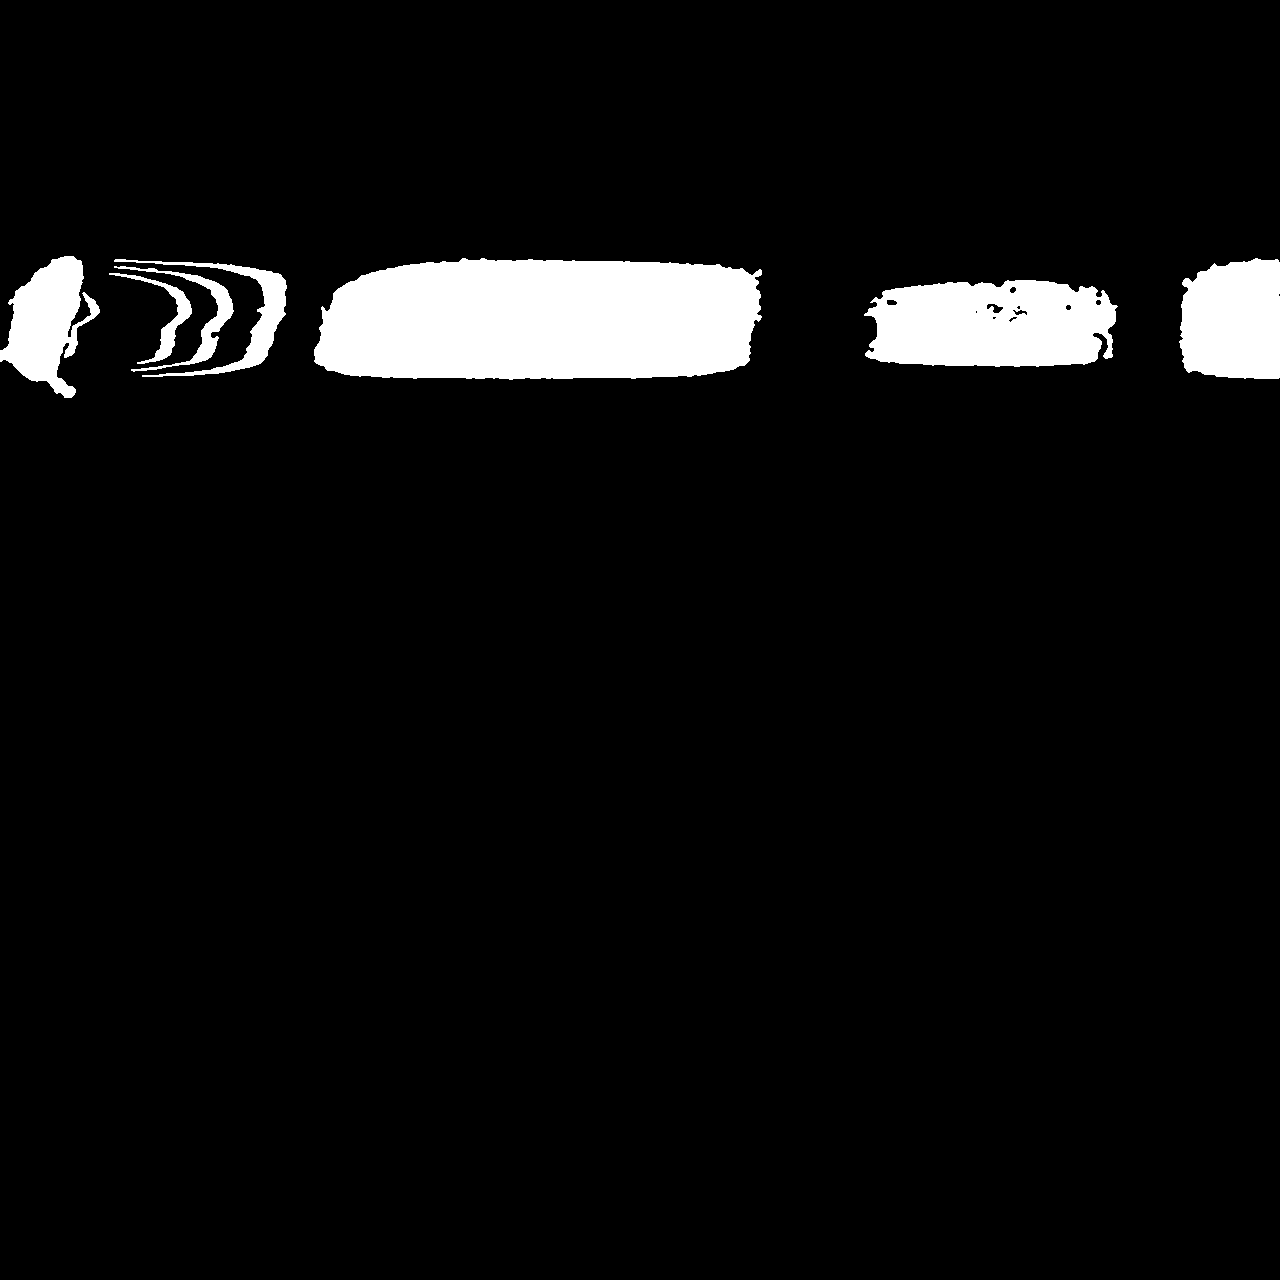
\includegraphics[width=\linewidth]{Maske.png}
		\caption{}
		\label{fig:mask}
	\end{subfigure}%
	\hspace{\fill}
	\begin{subfigure}{0.5\textwidth}
		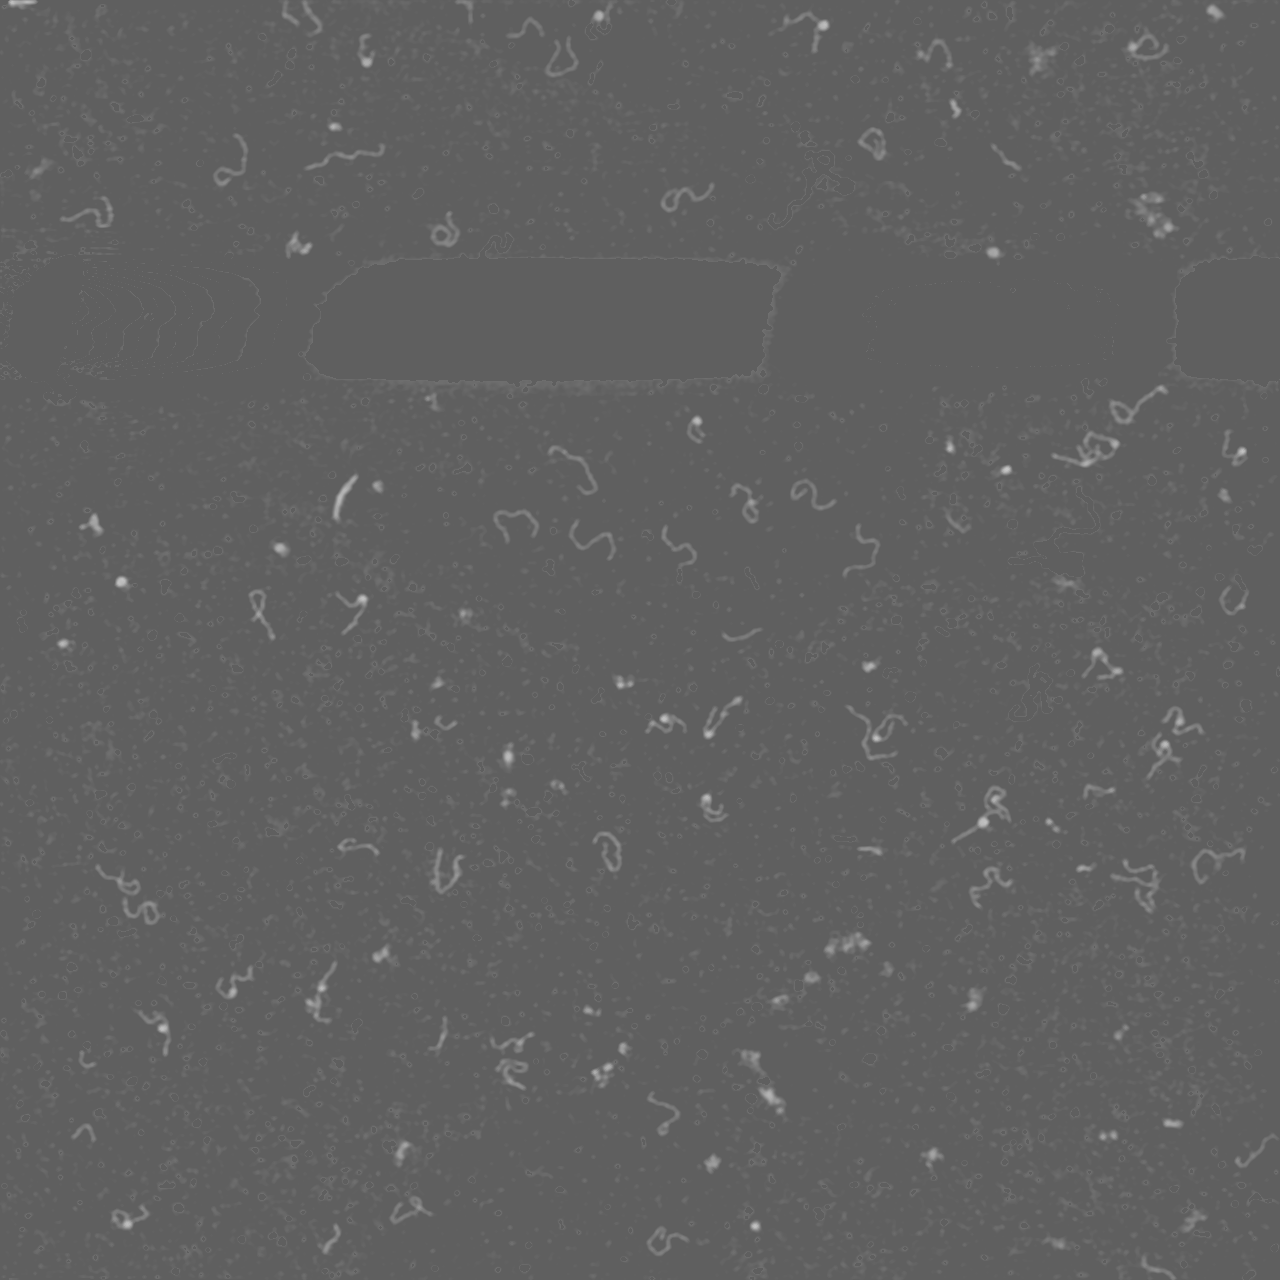
\includegraphics[width=\linewidth]{filtered.png}
		\caption{}
		\label{fig:filtered}
	\end{subfigure}%
	
	\caption{(a)Mask from binary image (b)Mask applied to original image}\label{fig:Process}
\end{figure}
This image is then used as a mask (compare Figure \ref{fig:mask}) which removes all non-DNA objects on the original image from step one.

This means subtract the detected regions on the mask from the original image and set them to the previous determined background level.
The result Figure \ref{fig:filtered} shows how the large outliers are removed and will therefore no longer contribute to the threshold in a negative way.
After this process a second threshold algorithm, in this case the moments threshold (see \ref{sec:Thresholding}), is applied to the original image. 
Duo to the previous steps the new calculated threshold is no longer influenced by background noise or polluted image regions.

In this case the new threshold is now at a intensity value of 111, compared to a intensity value of 135. Figure \ref{fig:compareThresh} shows the improvement in terms of recognized DNA objects on the sample image for type one noise as seen in Figure \ref{fig: Noise1}.
By using this approach it is now possible to analyze pictures with the first type of noise while they had to be discarded entirely before.


\begin{figure}[!htbp]
	\begin{subfigure}{0.5\textwidth}
		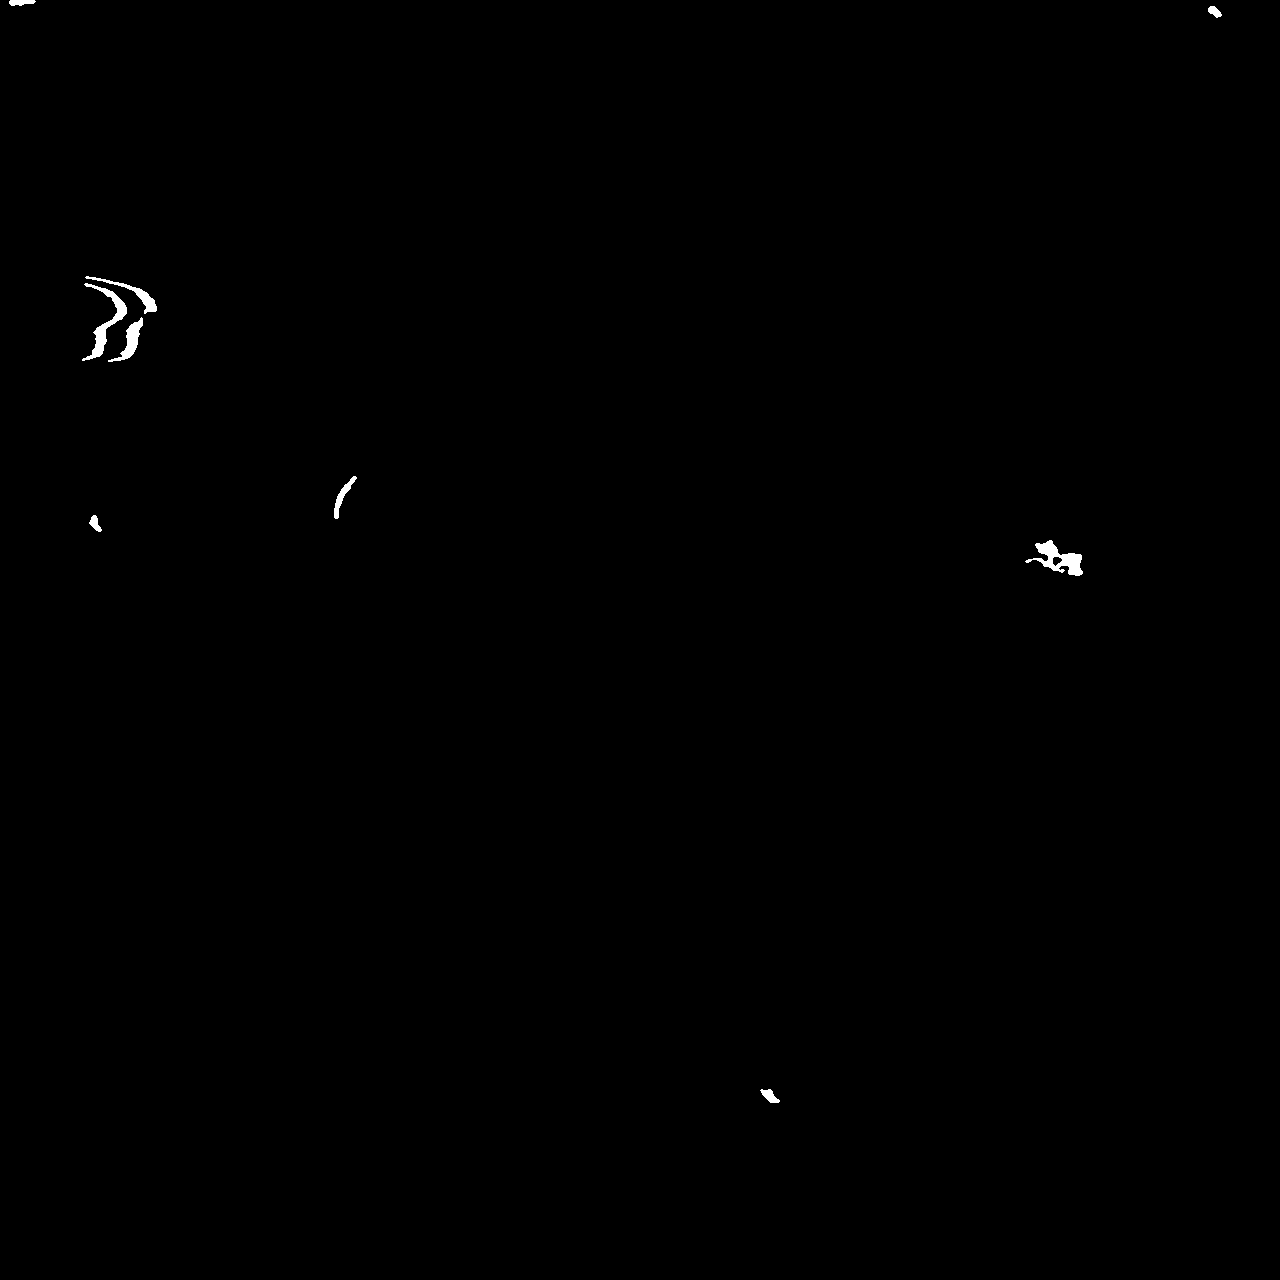
\includegraphics[width=\linewidth]{before.png}
		\caption{Before}
		\label{fig:bwbefore}
	\end{subfigure}%
	\hspace{\fill}
	\begin{subfigure}{0.5\textwidth}
		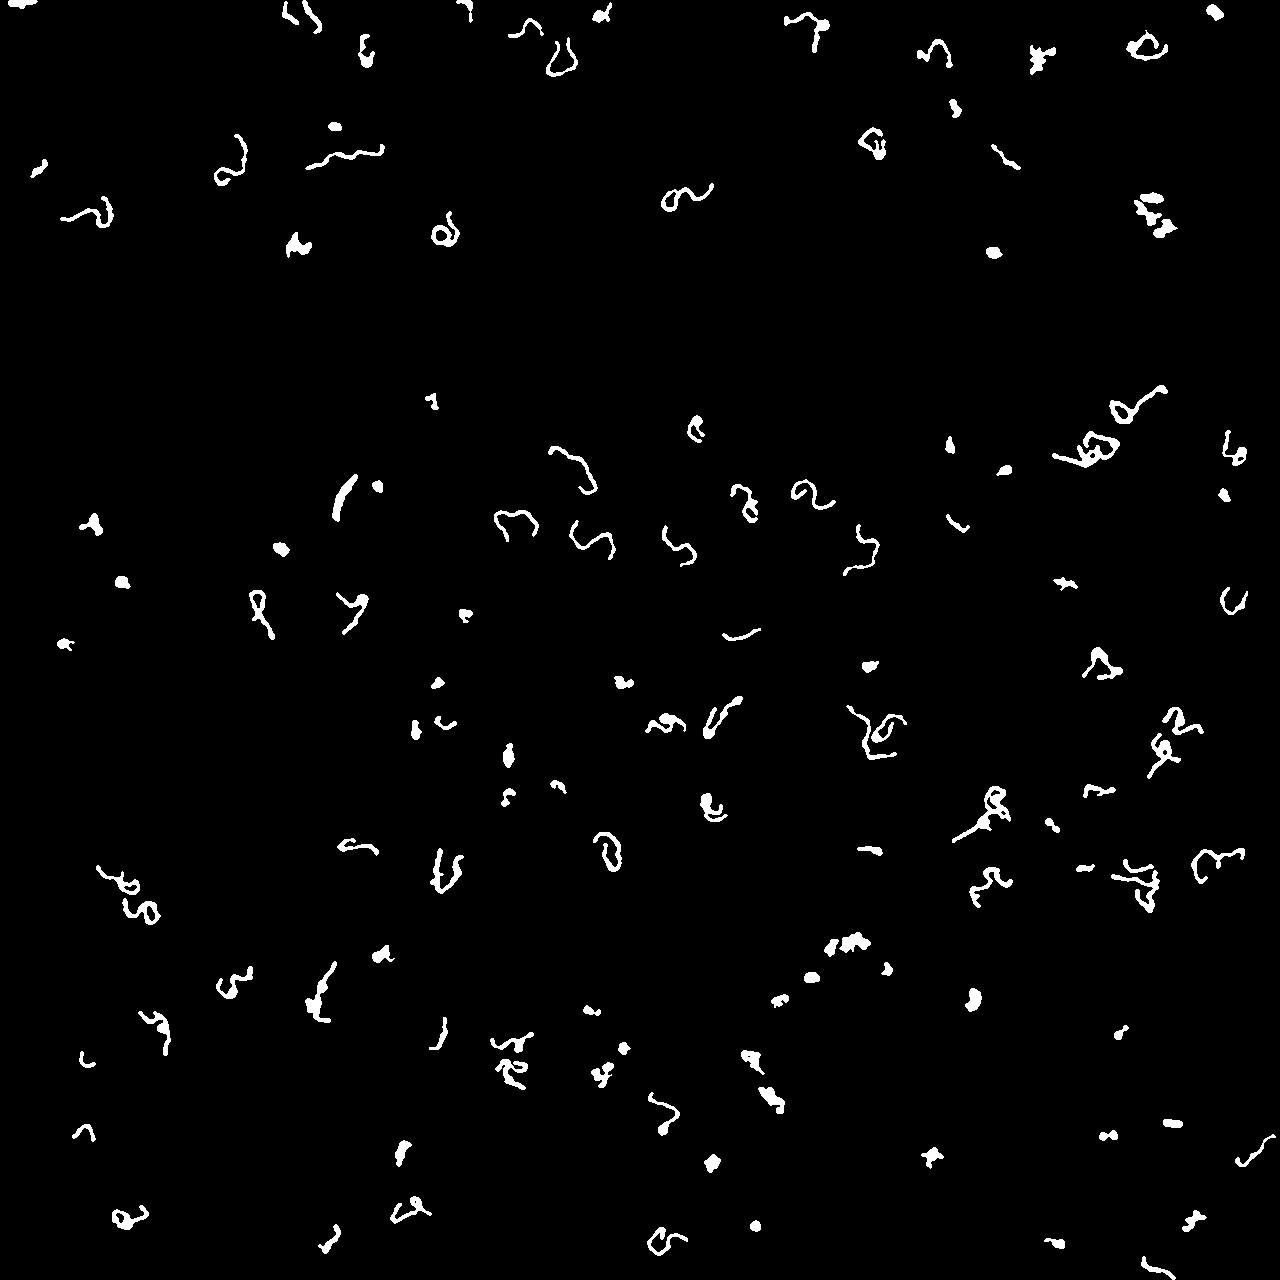
\includegraphics[width=\linewidth]{after.png}
		\caption{After}
		\label{fig:bwafter}
	\end{subfigure}%
	\caption{Comparison with previous method, noise type 1}\label{fig:compareThresh}
\end{figure}

\subsubsection{Limit Threshold}
The first two steps focused on keeping the noise and distribution of the height values in a tolerable range on image to image basis. The third and final step of this method aims at limiting the thresholds over the entire dataset.
For this technique a larger dataset of at least 50 images is required.
The histogram of all 105 test images shown in figure \ref{fig:HistogramThresholds} shows that step one and two already improve the thresholds to a smaller range.
Also, only thresholds, which were too high, have been limited by these steps since only outliers in the upper value range have been treated, while lower values have been set to a fixed background.
The newly calculated thresholds are in a range between 0.4 and 0.46 which corresponds to pixel values of 102 and 117.
Looking at the images with the highest and lowest thresholds, it turns out that they are still prioritizing lower respectively higher pixel values. This results in too small DNA-strands or false positive detections.
In order to limit the probability of these cases the permissible range for thresholds is reduced even further. This is achieved by only allowing thresholds in the range of 1.5 times the standard deviation around the mean of the distribution.
The range is thereby limited to: 
\[
[\bar X - 1.5 * \sigma, \bar X + 1.5 * \sigma] 
\]
\[
= [0.4345-1.5*0.0129, 0.4345+1.5*0.0129] 
= [0.4152,0.4538]\,  % Formel allgemein hinzufügen
\]
All values outside of this interval are set to the nearest boundary.



\begin{figure}[!htb]
	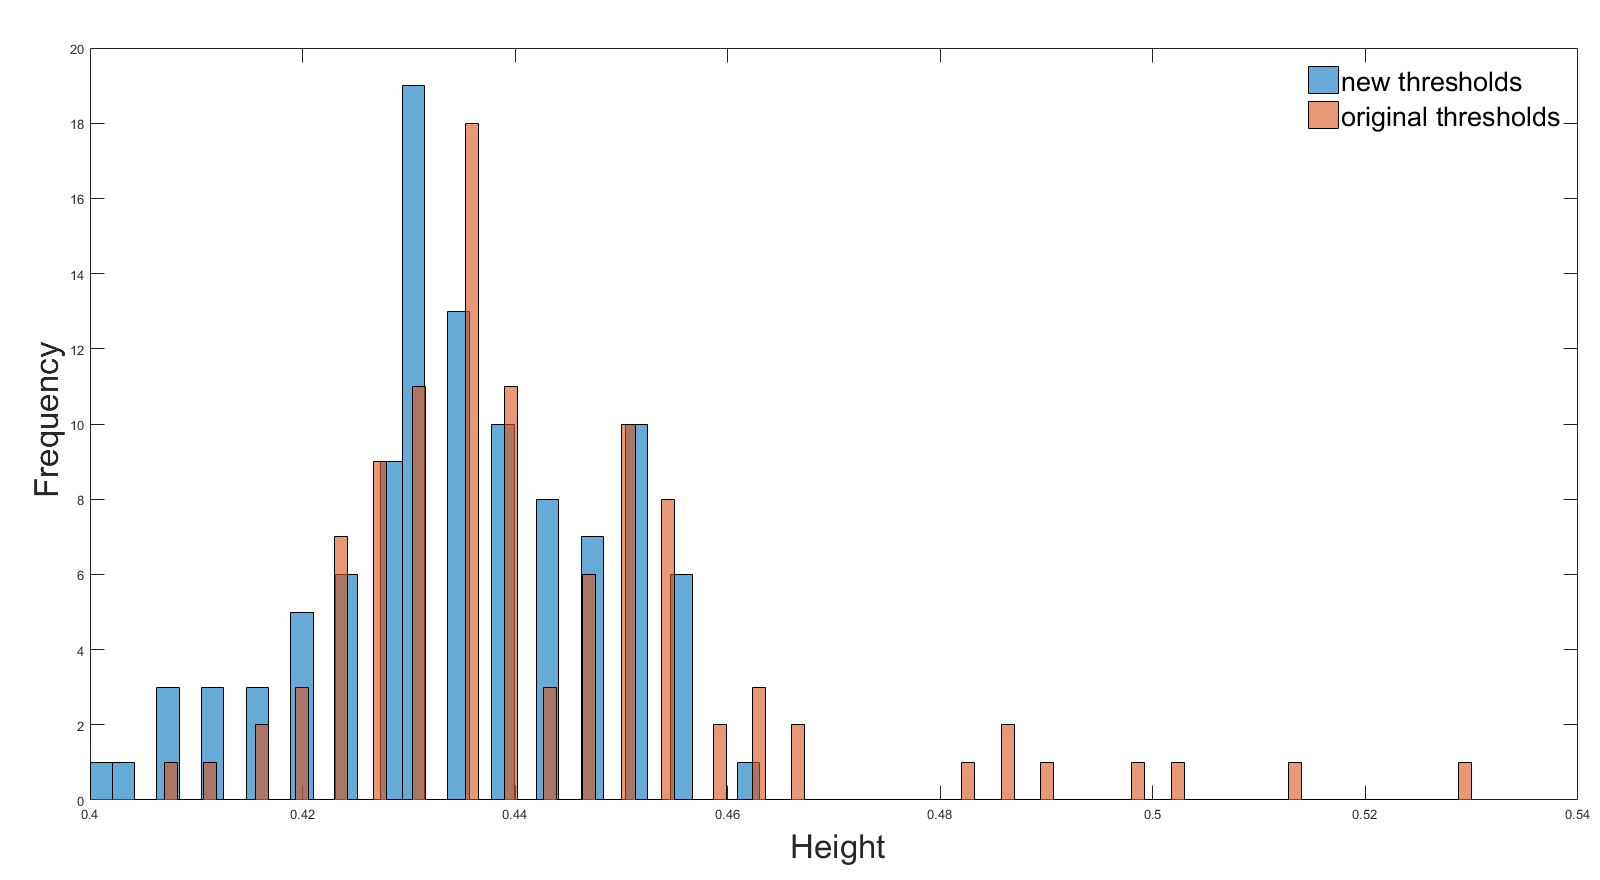
\includegraphics[width=1\linewidth]{thresholds.png}
	\caption{Threshold Distribution over the entire dataset (orange)before and (blue)after step one and two were applied}%formulierung ändern
	\label{fig:HistogramThresholds}
	\end{figure}
	As seen in figure \ref{fig:compareThresh} this method effectively detects and removes polluted image regions and ensures a high DNA-strand detection on images with noise type one.
Due to the nature and height field of noise of type two this approach can only limit false detections to a certain degree (see figure \ref{fig:compareThresh1}).
Although it was not expected to work on this kind of imperfections at all. While almost all DNA-strands are detected correctly some false positive still exist.
In conclusion, the proposed approach improves image quality and detection rate on very noisy images greatly while leaving already well processed images the way they are.

\begin{figure}[!htbp]
	\begin{subfigure}{0.5\textwidth}
		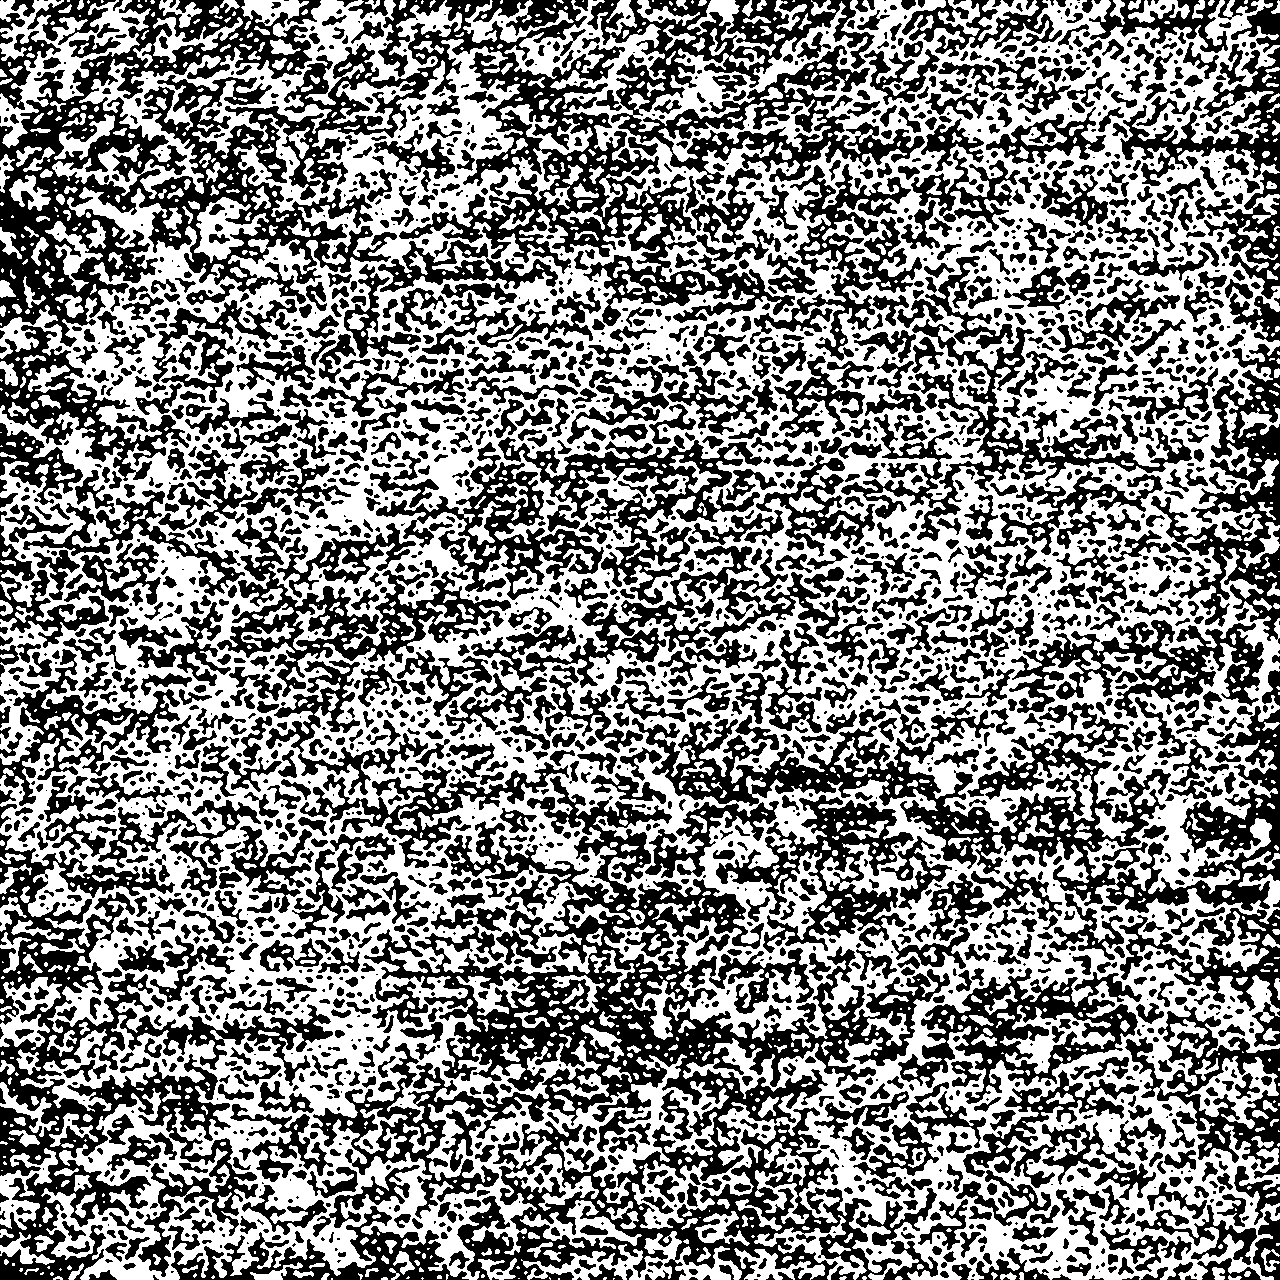
\includegraphics[width=\linewidth]{noise2before.png}
		\caption{Before}
		\label{fig:bwbefore}
	\end{subfigure}%
	\hspace{\fill}
	\begin{subfigure}{0.5\textwidth}
		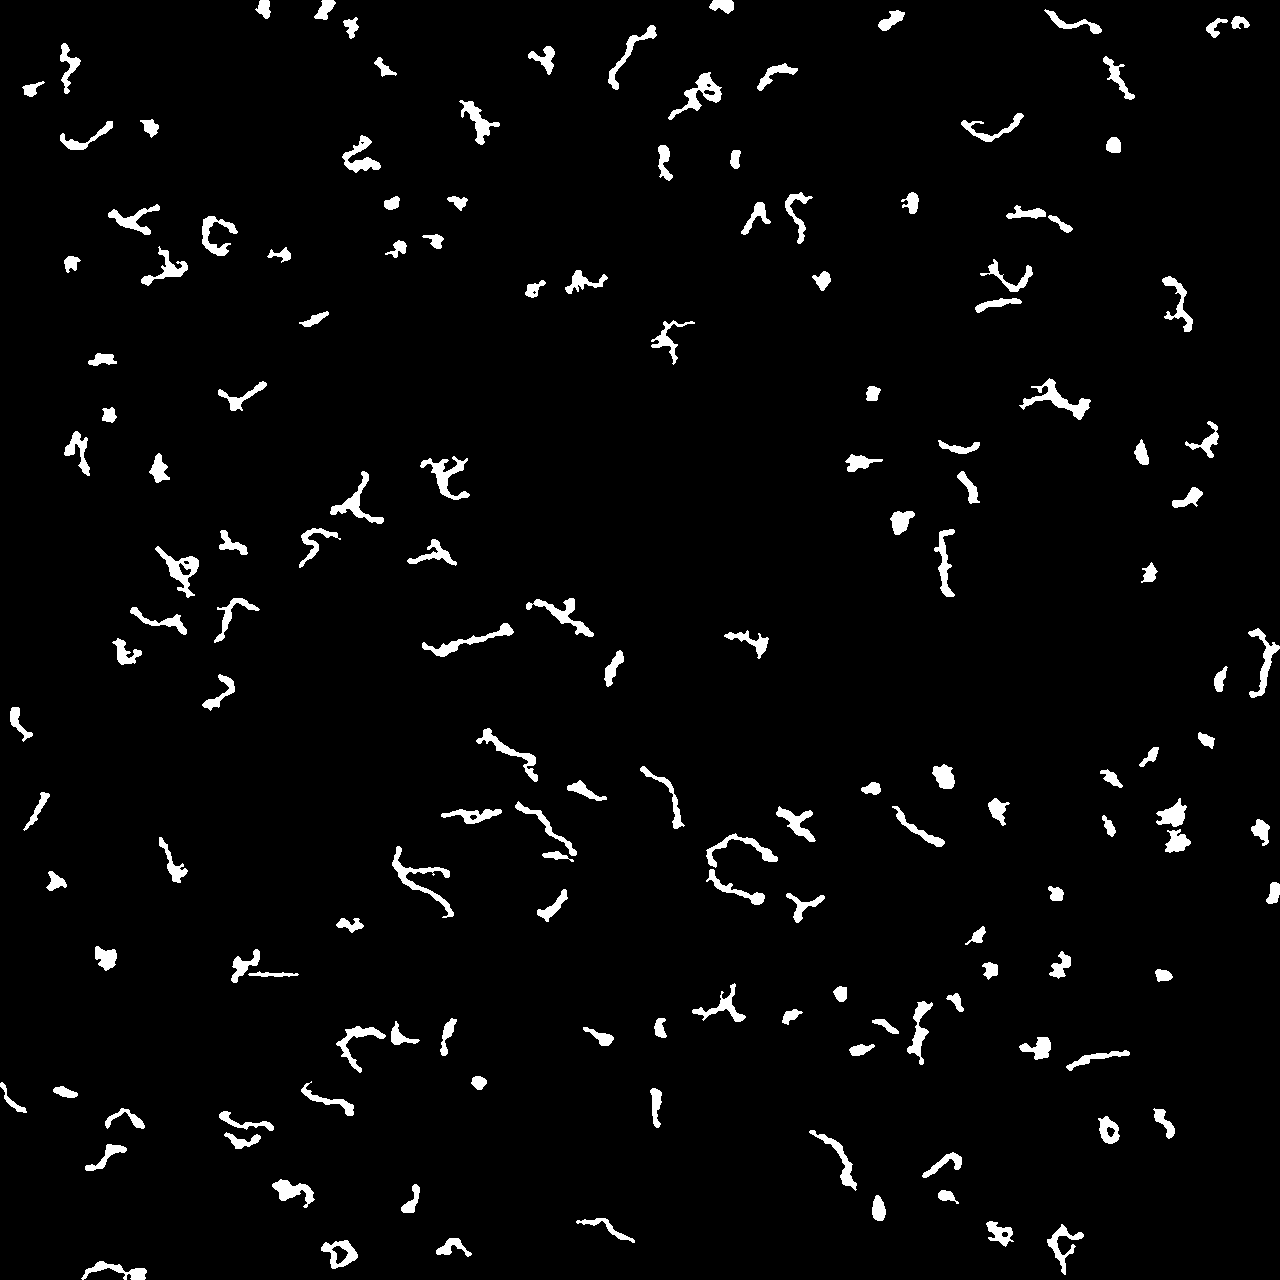
\includegraphics[width=\linewidth]{noise2after.png}
		\caption{After}
		\label{fig:bwafter}
	\end{subfigure}%
	\caption{Comparison with previous method, noise type 2}\label{fig:compareThresh1}
\end{figure}
\newpage
























\newpage

This is how you include figures:
\begin{figure}[htb]
	\begin{center}
		%\includegraphics[width = 0.7\textwidth]{041.png}
	\end{center}
	\caption{My Figure Caption.}
	\label{fig: example} % you need to include this to reference the figure afterwards
\end{figure}

This is how you reference a Figure: See figure \ref{fig: example}. \\
And this is how you reference a section: See section \ref{sec: Results}.


\subsection{Software Architecture}


\subsubsection{Processing Pipeline}
All images of the dataset are processed in a sequential way by the following nine steps:

\begin{enumerate}
	\item Denoise
	\item Filter
	\item Create binary image
	\item Detect nucleosomes %?
	\item Detect DNA strands 
	\item Calculate length of DNA strands
	\item Calculate angle between arms of a DNA strand if it possesses exactly one nucleus
	\item Save Results as CSV file
	\item Write processed image to disk
	
\end{enumerate}

At first every image is denoised by the OpenCV function fastNlMeansDenoising \footnote{http://docs.opencv.org/3.0-beta/modules/photo/doc/denoising.html} 
(\ref{Missing}) and passed on to the MATLAB main pipeline(see figure \ref{fig:PipelineDiagram}). % add rev
Inside the MATLAB pipeline an object-oriented approach is used.
This has the advantage that fields can be accessed easily like this:
\[
 imageObject.property
\]
Also the data is stored in a structured way which not only provides accessibility and modularity but also ensures maintainability and expandability.

Each image is instantiated as a object of the image class (figure \ref{fig:ClassDiagram}) which can hold essential properties such as a dnaList for detected DNA strands and numerous other information about the detected objects.
All data gathered during the process, such as the filtered image, the binary image, the thinned DNA strands, is stored as an instance variable.
Therefore all processing steps can be reviewed separately later on.
For example the denoising and filtering steps where improved by examining the intensity histograms of the pre-processed images.
Also different thresholds can be tested and assessed directly.
After being filtered by a median filter(see section \ref{sec:Filtering}) the lowPassFilter(see section \ref{sec:Adaptive Lowpass Filter}) function is applied to each image. 
To reduce noise even further the background is subtracted from the original image by the MATLAB imOpen \footnote{http://www.mathworks.com/help/images/ref/imopen.html} method.
The threshold distribution over the entire dataset is required in step three. Therefore all images have to be pre-processed by step one denoising and step two filtering before step three can proceed further. 
%In order to compute the threshold distribution, which is required in the third step,  all images have to be preprocessed by step 1 Denoising and step 2 filtering before being processed any further.
To create the binary image the adaptive thresholding function(see section \ref{sec: Adaptive Thresholding}) is used.
After that every image is scanned for nuclei by the findNuklei(see section \ref{sec: Nucleosome Detection})function which also stores them as centers and radii as fields of the current image instance.
Remaining objects are classified as DNA strands and therefore instances of the DNA class are created and saved in the DnaList field.
Each DNA strand is either stored as DNAFree if no attached nucleus was detected or as DNABound if at least one attached nucleus was detected.
\begin{figure}[!ht]
	
      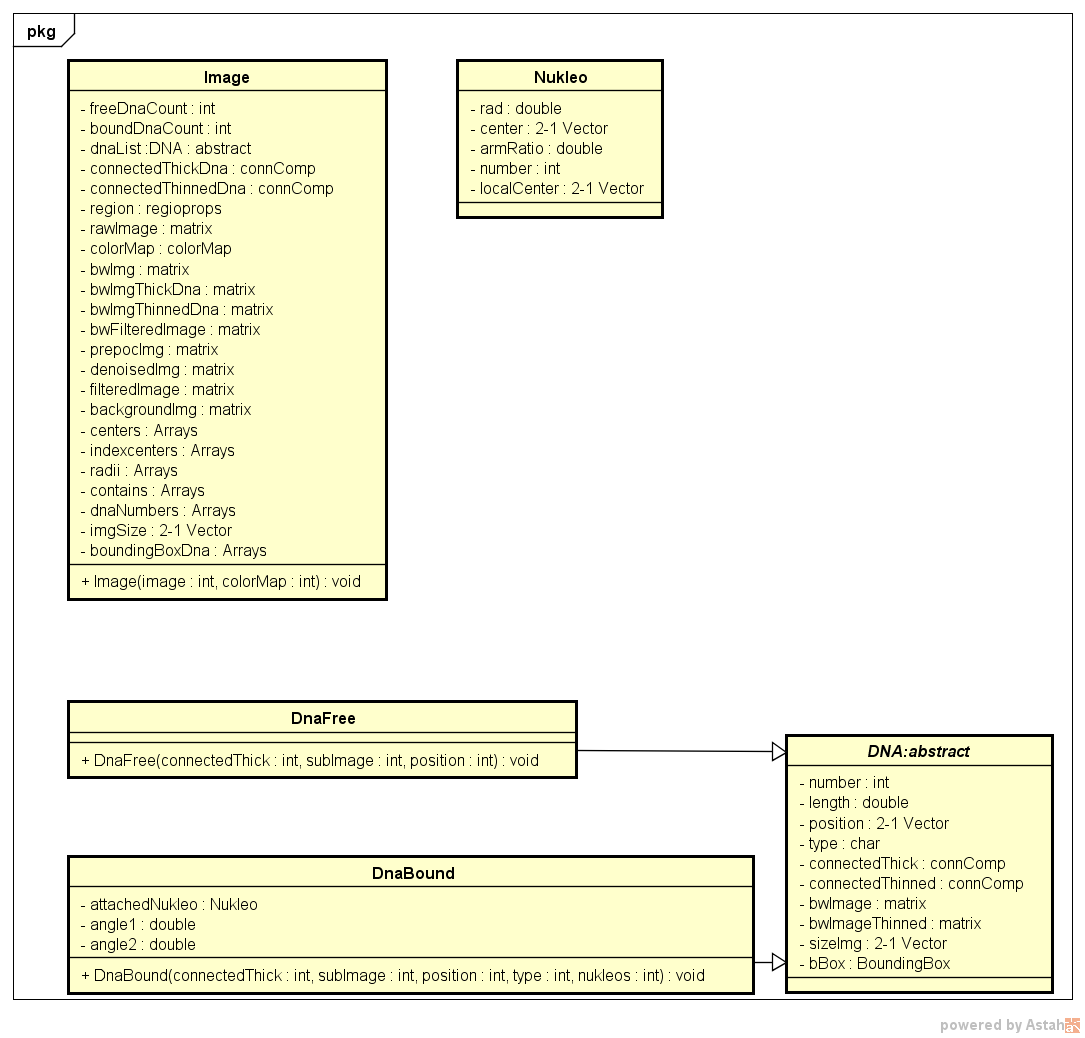
\includegraphics[width=1\linewidth]{ClassDiagram.png}
	
	\caption{class diagram of the pipeline of the program} %??
	\label{fig:ClassDiagram} % you need to include this to reference the figure afterwards
\end{figure}
Since all objects which persist after the three initial steps are classified as DNA strands, polluted image regions with a similar size are misclassified as DNA.
%a lot of noise which happens to have an acceptable size are misclassified as DNA as well.
To solve this problem DNA strands are marked as invalid if they do not meet certain criteria such as number of pixels, length and number of attached nucleus.
Only DNA objects with zero or one nuclei are permitted.
%Some Misshaped DNA objects are already marked as invalid during the findNuclii function. 
Step six, calculating the length of the DNA strands also marks DNA objects as invalid based on their length(see section \ref{}) % add missing rev
In order to calculate the length correctly it is necessary to thin the DNA strands first and remove the branches which arise during this thinning.
Step seven(Section \ref{sec:Angle Measurement})  calculates the angle between the two arms of the DNA strand, this only applies to DNA strands with an attached nucleus which are stored as DNABound in the dnaList variable.
DNA strands with more than one attached nucleus are marked as invalid.
The features length, angle, position on the image, position of the attached nucleus, radius of attached nucleus and the isValid flag are exported as a CSV file with filename,''meaning the name of the file''  \cite{UBHD-67466516},  [numberOfImage]-test.CSV.
\begin{verbatim}
@book{UBHD-67466516,
 author={Ludewig, Jochen and Lichter, Horst},
 title={Software Engineering},
 subtitle={Grundlagen, Menschen, Prozesse, Techniken},
 edition={3., korr. Aufl.},
 address={Heidelberg},
 publisher={dpunkt-Verl.},
 year={2013},
 pages={XXI, 665 S.},
 isbn={978-3-86490-092-1 ; 3-86490-092-1},
 language={ger},
 keywords={(s)Software Engineering},
 library={UB [Signatur:LN-U 10-13942::(3)] ; MA [Signatur:Ludew]},
}
\end{verbatim}

By exporting the isValid flag invalid DNA strands can be ignored during the evaluation but still persist in order to analyze difficulties, increase detection rate and improve performance.
At last all images created during this process, such as the binary image, are written to the disk.


\begin{figure} [!ht]
	
      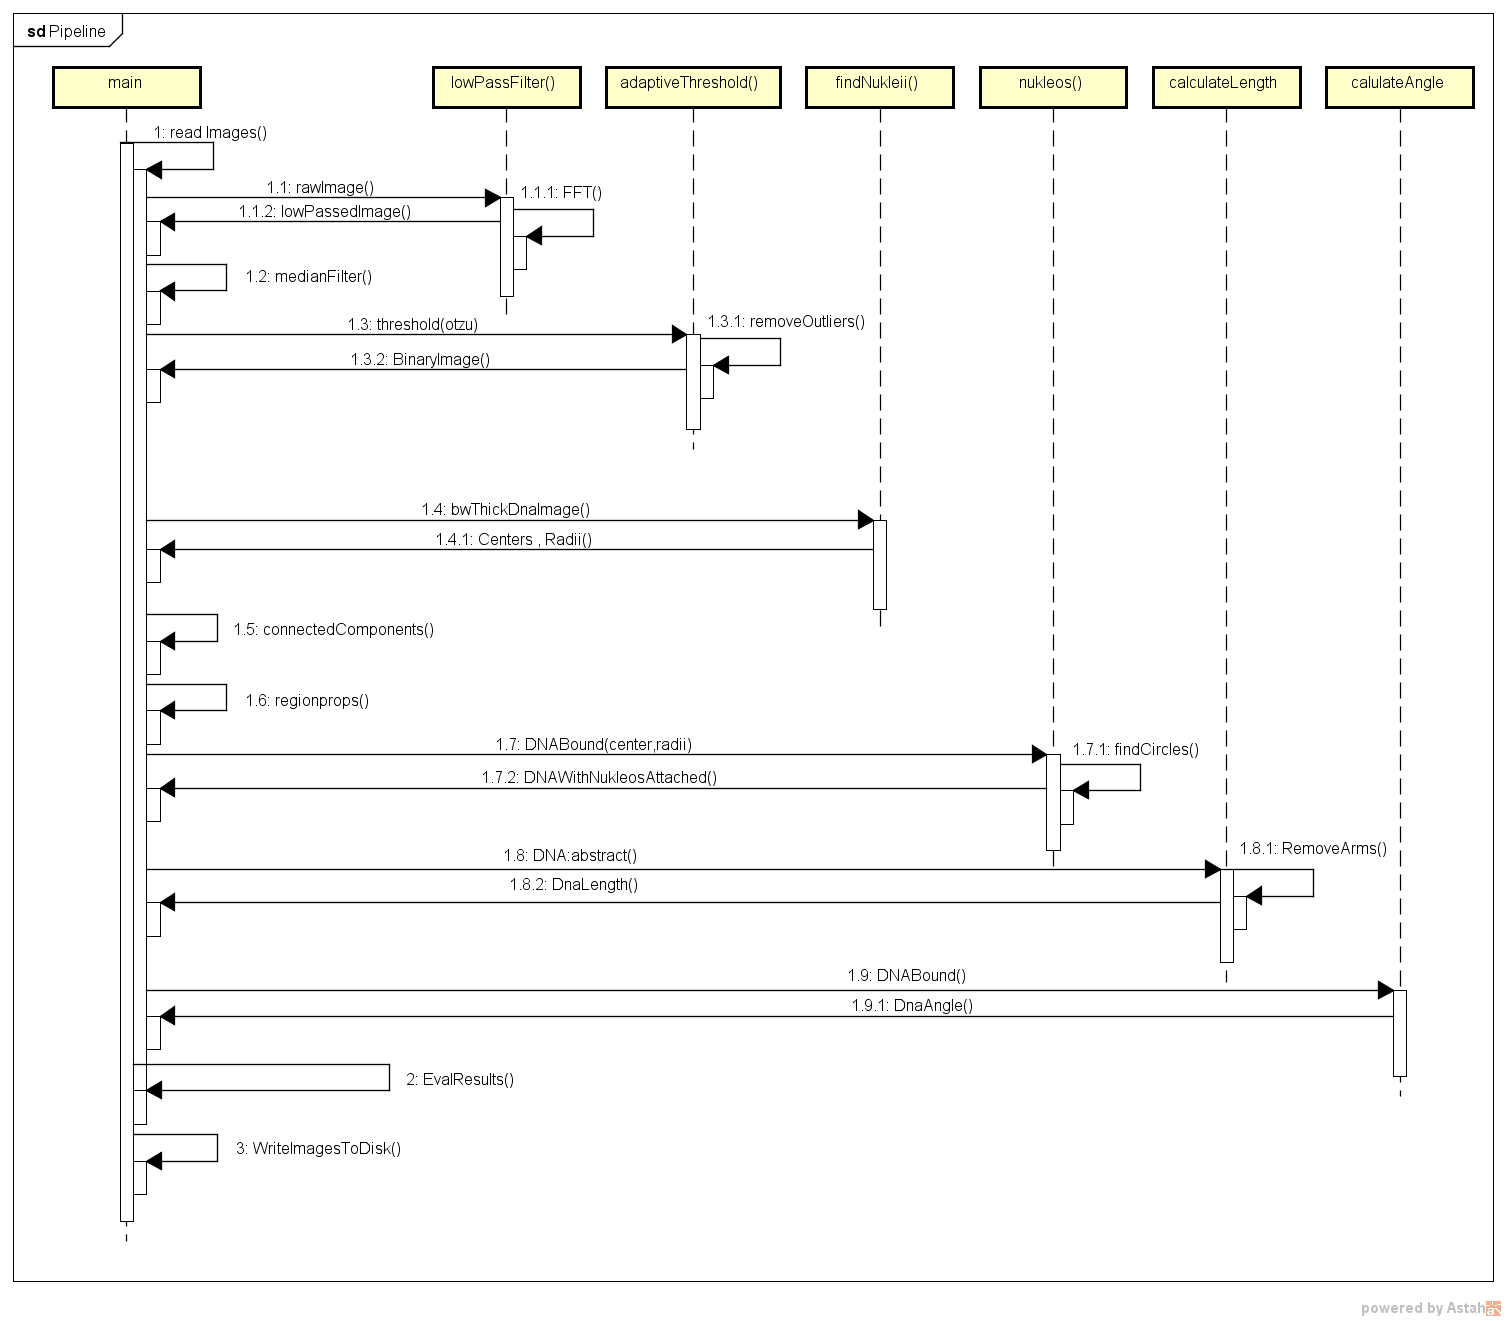
\includegraphics[width=1\linewidth]{Pipeline.png}

	\caption{sequence diagram of the pipeline of the program} %??
	\label{fig:PipelineDiagram} 
\end{figure}






\subsection{Algorithm}
\subsection{Runtime Optimization}
The main pipeline of the program (see section \ref{sec: Software Architecture}) takes up a total amount of 405 seconds for 105 images with a resolution of 1920x1920  on a standard workstation.
That means each image needs about 3.9 seconds to be processed from a raw image to a fully evaluated binary image with detected features as described in section \ref{sec: Software Architecture}.
3.9 seconds is already a short time period but the use cases for this kind of software usually contains processing thousands of these images.
Therefore ''the faster the better'' applies as long as the quality of the results is not reduced.
In order to optimize the runtime three steps were taken:

\begin{enumerate}
	\item optimize the use of MATLAB commands and indexing
	\item parallelize the execution of the pipeline and use multiple CPU cores
	\item use GPU for time consuming function calls
\end{enumerate}

To locate time consuming factors the MATLAB profiler \footnote{http://www.mathworks.com/help/matlab/matlab\_prog/profiling-for-improving-performance.html} was used.

At first inefficient array and matrix indexing like:
\[
list(find(list > value))
\]
was optimized by using logical indexing instead of the find function.
Also some for-loops could be accelerated by using vector or matrix operations which MATLAB handles very well.
Since five different developers worked on the program some values, such as the connected Components were calculated more than ones which could be improved by storing the values as an instance variable.
This process already improved the executing time from 405 seconds down to 350 seconds over the entire dataset(figure \ref{fig:OptWorkstation}) or from 3,9 seconds to 3,4 seconds per image.
\begin{figure}[!htbp]
	
      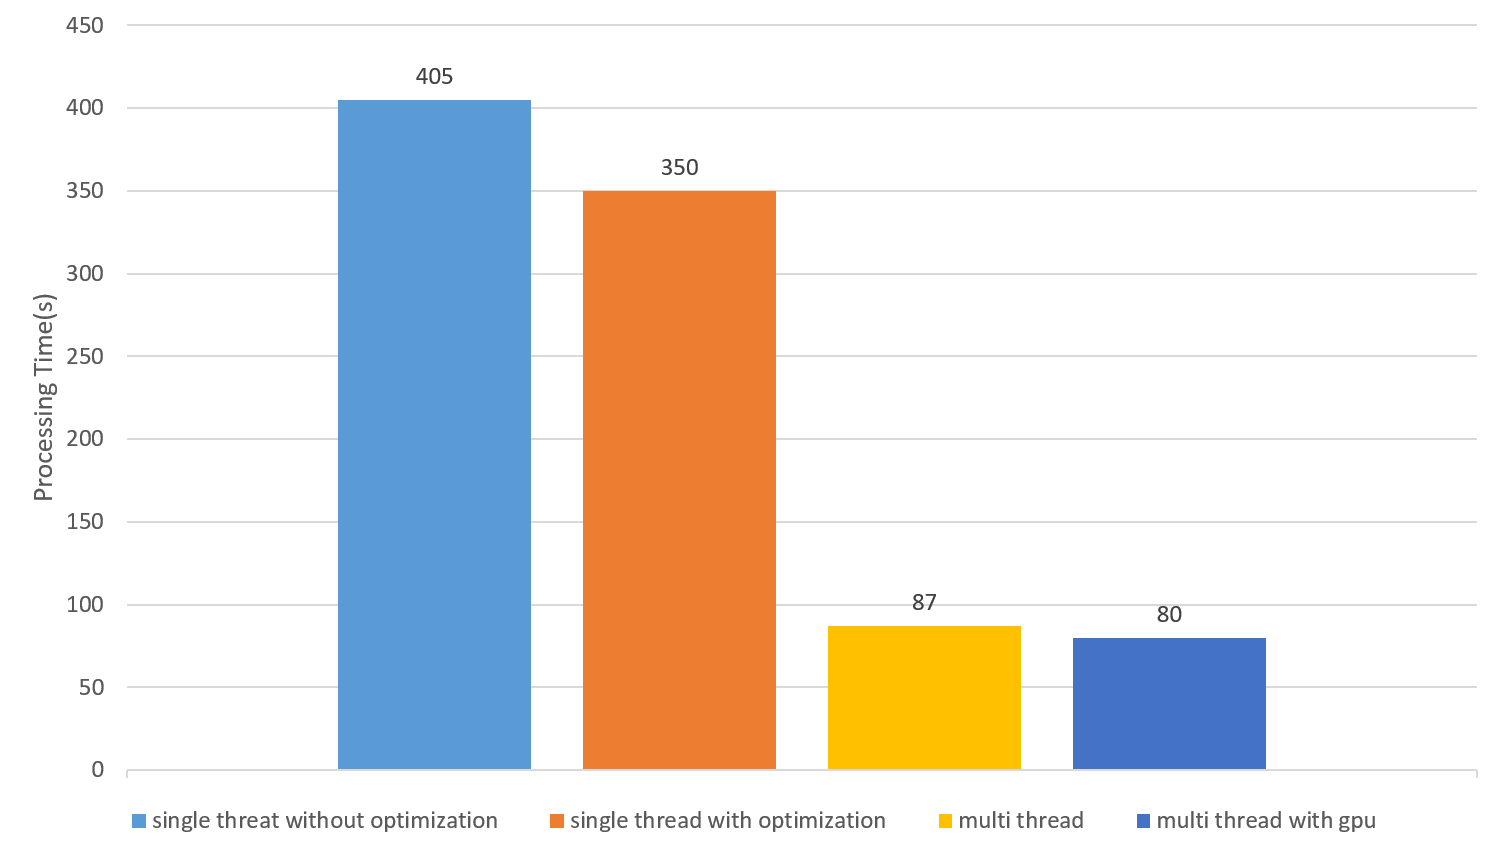
\includegraphics[width=1\linewidth]{OptWorkstation.png}

	\caption{Processing time over 105 images on a workstation (6 CPU Cores)} %??
	\label{fig:OptWorkstation} 
\end{figure}

As a second step the pipeline was parallelized such that multiple images could be processed at once.
Using the the parfor  \footnote{http://www.mathworks.com/help/distcomp/parfor.html}  command from the MATLAB parallel computing toolbox \footnote{http://www.mathworks.com/products/parallel-computing/} multiple workers/threads are started where each worker can handle one loop pass at a time.
The number of workers is limited by the number of CPU Cores available on the workstation used which were six in this case.
It is important to ensure that all workers only access disjoint parts of the data they work on.
Ideally the processing time is divided by six when not accounting for the multithreading overhead. Practically the processing time is quartered which means gong down from 350 seconds to 87 seconds over all 
and from 3.4 seconds to 0.83 seconds per image (figure \ref{fig:OptWorkstation}).
Such an improvement is only achievable when using large datasets of more than 100 images.
\begin{figure}[!ht]
	
      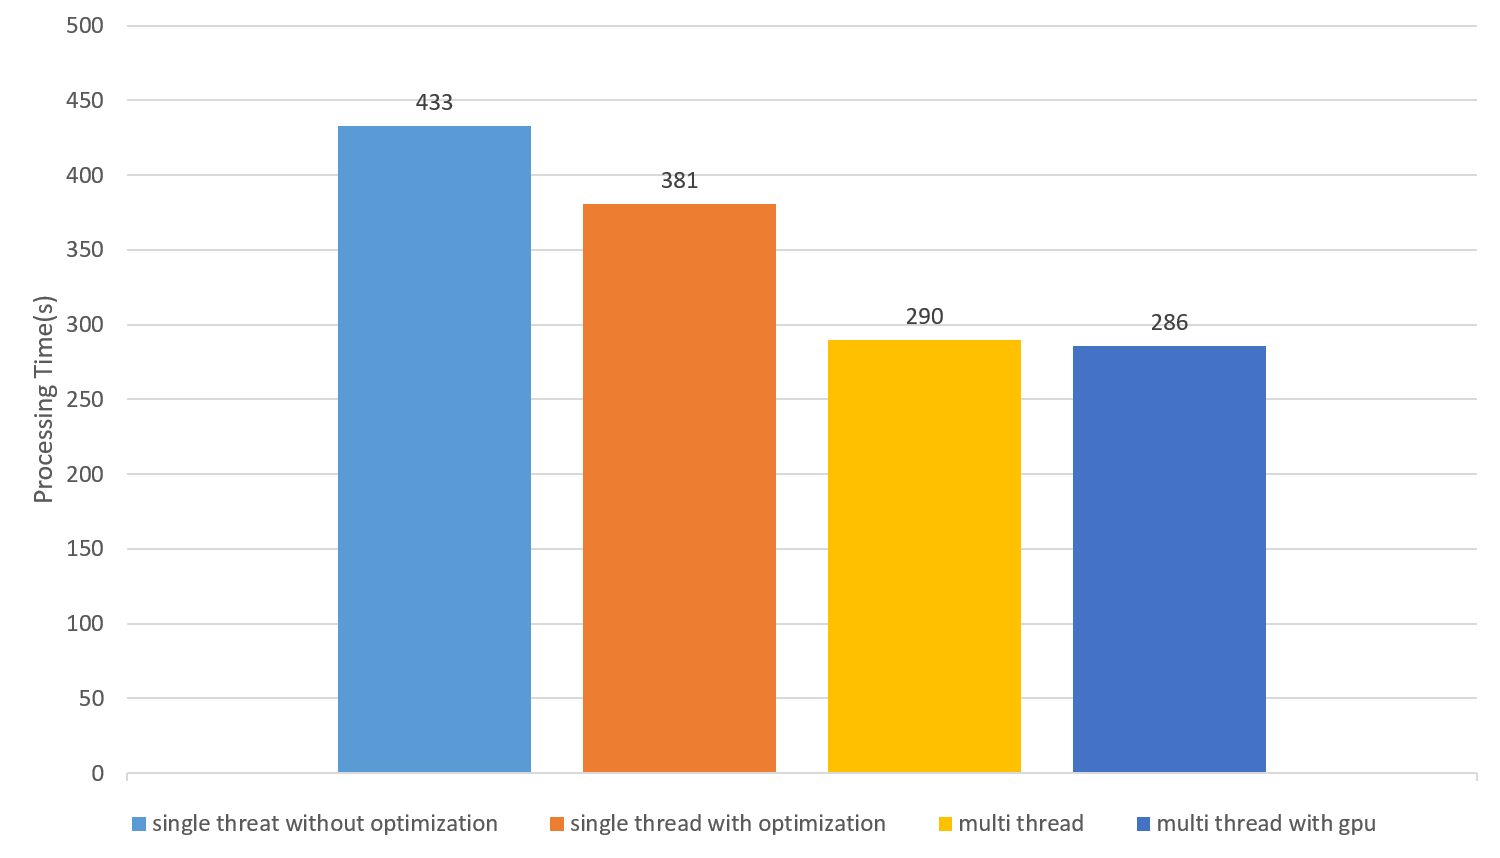
\includegraphics[width=1\linewidth]{OptLaptop.png}

	\caption{Processing time over 105 images on a consumer laptop (2CPU Cores)} %??
	\label{fig:OptLaptop} 
\end{figure}

The MATLAB parallel computing toolbox also provides GPU implementations for some functions such as bwmorph \footnote{http://www.mathworks.com/help/images/ref/bwmorph.html}
which is used during the thinning of the DNA strands (see section \ref{sec:Thinning}).
This approach reduced computation time from 87 seconds to 80 seconds respectively from 0.83 seconds to 0.76 seconds per picture.


    
All steps combined reduce execution time by 80.2 \% on a standard workstation.
Using a consumer grade laptop with two CPU cores holds far less potential for performance optimization.
Still, computing time can be reduced by 34\% over the entire dataset which corresponds to a performance gain of 1.4 seconds per image or an improvement from 433 seconds to 286 seconds for 105 images(figure \ref{fig:OptLaptop}).
These values improves by the size of the dataset because the multithread and GPU overhead is independent of the size of the dataset.








\subsection{Test Data Creation}
\section{Results}\label{sec: Results}
\subsection{Validation}
\subsection{Biological Significance}
\section{Discussion}
\section{Conclusion and Outlook}

\section{References}
%
\bibliography{sources}
\bibliographystyle{plain}

\end{document}
